\documentclass[tikz,border=2pt]{standalone}
\usepackage{amsmath,amssymb}
\usepackage{tikz}

\begin{document}
% Planned shortages: after replenishment the stock is s, it reaches zero after s/D and the
% backlog grows to y - s at the end of the cycle; the shortage cost is p times the red area.
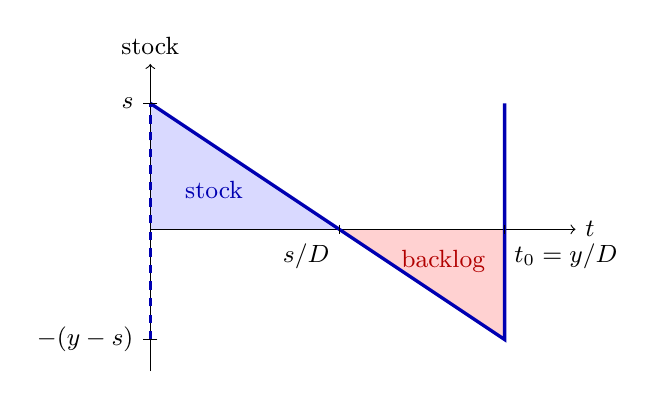
\begin{tikzpicture}[every node/.style={font=\small}, x=0.3cm, y=0.1cm]
	\fill[blue!15] (0,0) -- (0,16) -- (8,0) -- cycle;
	\fill[red!18] (8,0) -- (15,-14) -- (15,0) -- cycle;
	\draw[->] (0,0) -- (18,0) node[right] {$t$};
	\draw[->] (0,-18) -- (0,21) node[above] {stock};
	\draw[blue!70!black, very thick] (0,16) -- (15,-14) -- (15,16);
	\draw[blue!70!black, very thick, dashed] (0,-14) -- (0,16);
	\draw (0.3,16) -- (-0.3,16) node[left] {$s$};
	\draw (0.3,-14) -- (-0.3,-14) node[left] {$-(y-s)$};
	\draw (8,0.6) -- (8,-0.6) node[below left] {$s/D$};
	\draw (15,0.6) -- (15,-0.6) node[below right] {$t_0=y/D$};
	\node[blue!70!black] at (2.7,5) {stock};
	\node[red!70!black] at (12.4,-4) {backlog};
\end{tikzpicture}
\end{document}
